\chapter{Background and Research Context}
\label{chap:background}

% ============================================================================
% CHAPTER PURPOSE -- HIGH PRIORITY
% Establish the motorsport and academic context required to understand the
% undercut problem. The reader should finish this chapter understanding:
%   1. why pit stop timing matters in modern Formula One;
%   2. how tyre behaviour creates an undercut opportunity;
%   3. what stay out, undercut and overcut strategies mean in race terms;
%   4. what relevant work already exists; and
%   5. the specific gap addressed by this project.
%
% Keep equations, model variables and software design out of this chapter.
% Those belong in Chapters \ref{chap:model} and \ref{chap:implementation}.
% ============================================================================

\section{Formula One Race Strategy}
\label{sec:race-strategy-background}

% HIGH PRIORITY -- approximately 0.5--1 page.
% Explain only the history needed to reach the modern tyre-strategy problem:
% - early emphasis on reliability, fuel and mechanical preservation;
% - refuelling as a strategic variable;
% - the 2010 refuelling ban and increased significance of tyre timing;
% - modern strategic decisions under mandatory tyre-compound rules.
% Cite regulations and authoritative motorsport/strategy sources.
% Avoid a broad history of F1 that does not support the research problem.

Since the beginning of the Formula One World Championship (F1) in 1950, races have been won and lost through a combination of vehicle performance, driver performance and strategic decision-making. The relative influence of each factor has changed as the technical and sporting regulations have evolved.

Early pit stops were frequent and done out of mechanical necessity. Cars were less fuel efficient and did not have tanks which could hold a race's worth of fuel, especially given that races were initially raced at ~500 kilometres rather than the maximum 320km set in 1971 \cite{F1Technical2009RaceDistance} and still used today. They were uncoordinated and dangerous affairs; fuel poured in from jerry cans risking dangerous blowback \cite{MotorSport1994Refuelling}, central wheel nuts secured with hammers \cite{Driver612022WheelNuts}, and upwards of a minute stationary while the mechanics worked. The time lost typically meant that race strategy was of minimal concern as it was heavily outweighed by practicalities.

Strategic pit stop strategies still occurred but were also far more simplistic, typically only considering the extra weight of fuel and newer tyres. The earliest example of the "tactical" pit stop is considered to be Juan Manuel Fangio in the 1957 German Grand Prix, who pitted on lap eleven and emerged fifty one seconds behind two Ferraris, before repeatedly setting fastest laps of the race and breaking the circuit records, before overtaking both cars on the final lap to secure his fifth World Championship, and his twenty fourth and final race win \cite{RaceFans2008PitStops}. This would be expanded into what more closely resembles a modern pit stop, with dedicated engineered equipment and tactical consideration, by Brabham at the 1982 Austrian Grand Prix who arrived with "what looked like beer kegs, huge diameter hoses, a blue chimney and a system to power the wheel guns" \cite{Automobilist2024PitStopRevolution}. The kegs were pressurised fuel delivery systems, capable of pumping 130 litres of fuel in three seconds, while the blue chimney was the predecessor to tyre blankets, with a gas blower heater at the bottom and small windows to check temperatures. Patrese's car would not finish the race, but it had demonstrated the effectiveness of pit stop equipment and influenced various regulations, such as the banning of refuelling from 1984-1994 \cite{FIA1984TechnicalRegulations} and from 2010 \cite{FIA2010SportingRegulations}. 

\begin{figure}
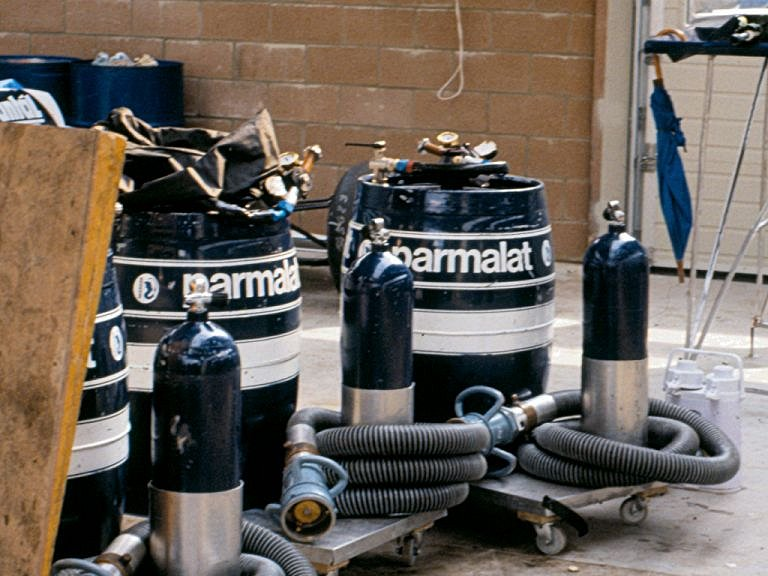
\includegraphics[width=\textwidth]{Figures/1_brabham-fuel-barrels}
\caption{Brabham's fuel tanks used to refuel during the 1982 Austrian Grand Prix. Source: \cite{Substack2024BrabhamFuelBarrelsImage}. Reproduced for educational purposes only.}
\label{image:brabham_fuel}
\end{figure}

Despite all the advances in technology, refuelling and tyres continues to be the cornerstone of race strategy. Every extra lap's worth of fuel adds weight to the car, reducing acceleration and increasing breaking distances, meaning every kilogram needs to be carefully considered. This effect is carefully calculated based on the characteristics of the car and will be a variable of race strategy optimisation models. For practical race strategy applications, this is typically approximated as linear over a stint and is considered independent from tyre degradation effects \cite{Cappello2026TyreDegradation}. Despite the current ban on mid-race refuelling applied in 2010 \cite{FIA2010SportingRegulations} these effects must be considered during non-race sessions, to find the true pace of a car independent of fuel in practice, and to achieve the lowest possible lap time without risk of running out of fuel and stopping on track to end a driver's qualifying session early. Fuel strategy represents a trade-off between lower vehicle mass and fuel saving requirements. Starting with less fuel reduces the lap time penalty associated with carrying additional mass but requires the driver to recover the fuel deficit through techniques such as lift-and-coast or reduced throttle application. Carrying additional fuel removes or reduces this requirement, allowing the driver to maintain a more aggressive driving style throughout the stint at the expense of a higher initial vehicle mass.

Tyre compound and degradation are the main strategic component of modern F1. Before the 1990s choice of tyre was more of an afterthought, with teams using mass produced road tyres which were poorly designed for racing situations - various estimates suggest ~30\% of race retirements during the 1950s and 60s were caused by tyre failures \cite{GrandPrix2472023TyreEvolution}. Various advances were made, particularly in the 1970s, with the introduction of radial tyre construction and the differentiation between slick and grooved tyres for dry and wet situations, but these did not typically provide strategic variety [x - footnote - Hunt / Lauda 1976 Japan] as each team would adopt the latest technologies. The multiple manufacturers eventually reduced during the 1990s and 2000s to various combinations of Goodyear, Bridgestone, and Michelin, which led to teams choosing dedicated tyre manufacturers which could tailor products to their needs, such as the alliance between Bridgestone and Scuderia Ferrari \cite{Bridgestone2002FerrariPartnership,Crash2005FerrariBridgestone}, and resulted in "Tyre Wars" between the manufacturers and their associated teams [x - find source] as each developed proprietary rubber compounds [x] and affected teams' abilities to compete such as the infamous 2005 Indianapolis Grand Prix where all Michelin tyre runners were required to retire due to safety concerns. The Federation Internationale de l'Automobile (FIA) eventually mandated single tyre manufacturers and introduced the modern range of dry compound tyres. 

The availability of each has varied over the years, peaking with the affectionately termed "Tyre Rainbow" of 2018 with seven distinct dry tyre compounds, before settling on picking three compounds from a pool of five (rated C1, softest, to C5, hardest) to serve as soft, medium, and hard tyres for each race in 2019 and is still the availability today. The different compounds are made of different blends of chemicals, including rubber, carbon black, silica, oils, and resins to form the chemical properties of the tyre which modify how it behaves under various lateral and longitudinal G-forces, how quickly it degrades, and how it behaves at racing temperatures.

\subsection{The Modern Pit Stop Decision}
\label{subsec:modern-pit-decision}

% HIGH PRIORITY.
% Explain the decision facing a team during a dry race:
% - continue on the current tyre;
% - stop earlier than a competitor;
% - stop later than a competitor.
% Introduce track position, tyre performance and rejoin traffic as interacting
% considerations, but do not define model parameters yet.
% End by explaining why the decision is difficult: the outcome depends on
% several time-varying and partially uncertain effects.

During a standard dry race, strategy teams need to make decisions about when the best time to commit to a pit stop is that will have the best overall impact to the driver's race time and position. A driver is required to use two distinct compounds of dry tyres under the 2026 regulations \cite{FIA2026SportingRegulations} at time of writing, meaning that at least one pit stop is required during a standard race for every driver [x - footnote - red flag rules]. This creates a set of variables that can affect the targeted lap for a pit stop.

Firstly is tyre degradation. Each tyre has an expected number of laps in its useful life as detailed in \cref{subsec:tyre-degradation-background}. If a driver stops too early in a race, the new tyre may not last until the end of the race or the next intended pit stop lap. Conversely, leaving a pit stop too late may mean the current tyre runs out of useful life causing severe time loss before the driver can return to the pits. Tyre behaviour is also a factor to consider - softer tyres typically reach their peak grip phase quicker, meaning a driver loses less time controlling a car with less grip on colder tyres. 

Competitors on the track also contribute to ideal timing for a pit stop for several reasons. Two drivers in F1 close to each other on track, on tyres of the same age and of the same tyre compound, have no differentiating factors to separate them except driver ability. However, the driver behind is driving through "dirty air", where the air coming off the car behind is washed outwards in spirals and vortexes, and does not behave smoothly providing consistent downforce as it does for the car at the front \cite{RacecarEngineering2020DirtyAir}. This makes it more difficult for the driver behind to follow closely or approach to overtake without assistance, as their car behaviour is unpredictable, leading to attempts to minimise its effect by technical regulations \cite{FIA2021ShapeThingsCome}. This is demonstrated in \cref{image:dirty_air_sim} with clean air coming in straight at the front, and appearing wavy as it comes off the back of the car. 

\begin{figure}
    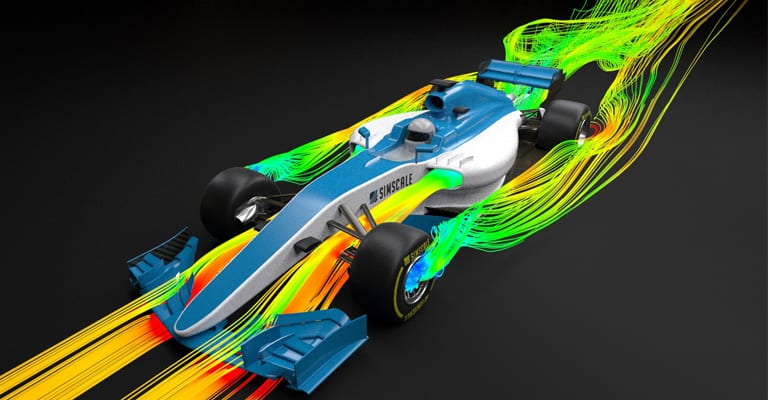
\includegraphics[width=\textwidth]{Figures/1_dirty_air_sim.jpg}
    \caption{Visualisation of the turbulent wake ("dirty air") produced behind a Formula One car. Source: \cite{SimScale2016FrontWingOptimisation}. Reproduced for educational purposes only.}
    \label{image:dirty_air_sim}
\end{figure}

By taking a pit stop, the driver behind may come out into a gap in traffic, giving them the clean air and they can go faster. They also don't lose time from defending position against drivers behind them. The reverse is also applicable; the driver behind can stay out if the driver ahead pits, freeing them into clean air and drive faster. Traffic around the pit stop procedure can impact whether this will be an effective strategy, as a driver can exit the pit lane into no gap and be unable to overtake slower moving traffic that was previously behind them.

These, amongst several other factors, are wildly fluctuating variables that impact whether a pit stop is a viable option to improve the driver's race time or to get in front of a competitor. Pure speed is not the only important outcome of a pit stop; track position can be equally important if the characteristics of a racetrack make overtaking difficult. All of these can change in a second and make a pit stop attractive or not, meaning it is incredibly difficult for the strategy engineers to attempt to predict the future and choose the best course. These variables led to the development of tactical pit stop strategies, such as the undercut.

[x - TODO - Why undercuts are difficult to analyse in retrospect, review below]

Although the outcome of an undercut is visible in historical timing data, determining why it succeeded is considerably more difficult. The observed lap time difference combines tyre degradation, compound performance, warm-up behaviour, traffic, driver pace and numerous interacting effects that cannot be directly separated. A useful engineering model must therefore estimate the contribution of each factor individually.
 
\subsection{Rise of the Undercut}
\label{subsec:rise-undercut}

% HIGH PRIORITY.
% Explain how high-degradation tyres and restricted compound allocations made
% undercuts prominent in modern F1. Cover:
% - an earlier stop exchanges temporary track position for fresher-tyre pace;
% - the gain is realised during the offset laps before the rival stops;
% - the undercut may fail through poor warm-up, traffic or insufficient delta.
% Use one or two concise historic examples if well sourced.
% Do not yet calculate the gain.

An undercut in motorsport is a strategic move which involves pitting earlier than an opponent ahead on track. This puts the driver onto fresh tyres, likely to be faster than an opponent's degraded tyres. This difference allows the driver to go faster on the out lap than the driver who was previously ahead. Even if that driver pits the following lap, this time lost means they may exit the pit lane behind the attacking driver, or so close that the driver who pit first has warmer tyres and is able to use this advantage in the corners to overtake immediately. 

The 1998 Hungarian Grand Prix is widely regarded as one of Formula One's defining strategic victories, with Ferrari using an aggressive three stop strategy to undercut the leading McLarens and secure victory despite limited overtaking opportunities \cite{Formula12020Hungary1998}. While strategic pit stop timing has influenced Formula One for decades, the removal of refuelling in 2010 placed even greater emphasis on tyre performance, making the undercut a central tactical consideration in modern race strategy.

It is important to note that this is not a guaranteed method of overtaking. Poor tyre warm-up on the outlap, the impact of traffic (both for the attacking and target driver), or attempting the undercut from too far back (so unable to close the gap even in perfect conditions) can all cause the attempt to fail and the situation on track remains unchanged. The driver ahead may also choose to stay out and build up tyre delta. When they eventually do pit, they'll have tyres several laps newer than the driver who attempted the undercut. Even if they are behind, their newer tyres will give an advantage attempting to overtake, meaning the advantage of the undercut is countered.

\section{Tyre Behaviour Relevant to Strategy}
\label{sec:tyre-behaviour-background}

% This is a focused literature-backed section, not a tyre-engineering textbook.
% Explain only the tyre behaviour needed to justify the later model.

\subsection{Tyre Compounds and Performance Trade-Off}
\label{subsec:tyre-compounds}

% HIGH PRIORITY.
% Explain the relative pace/durability trade-off between nominated compounds,
% without assuming that the soft is always strategically preferable.
% Mention that the actual performance delta is event- and condition-dependent.
%
% SUGGESTED FIGURE 1.1:
% Conceptual compound pace versus durability diagram.
% Mark as conceptual rather than measured data.

 \cref{fig:1_conceptual_tyres} shows how different tyre compounds affect tyre life and behaviour at an abstract level. A softer tyre typically has more grip, being able to warm up to racing temperatures more quickly and mould to the granularity of the road, but degrades more quickly as the rubber is pulled apart by the tarmac, making it the preferred tyre for single-lap pace in qualifying. The harder tyre is the reverse, being longer and more durable while sacrificing higher grip, making it more suitable for longer race stints \cite{RaceTeq2024TyreDegradation,Taylor2020FrictionRacingTyres,RacecarEngineering2020TyreGrip}.

\begin{figure}[htbp]
\centering
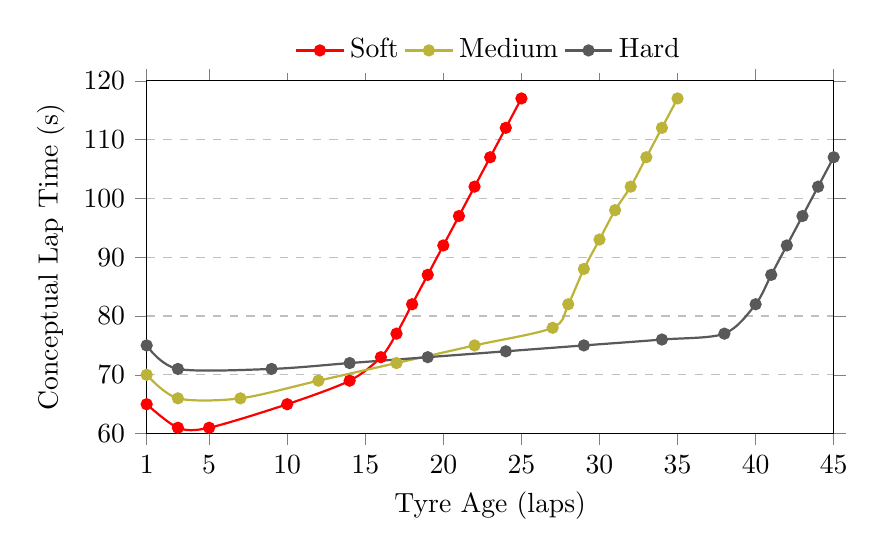
\begin{tikzpicture}
\begin{axis}[
    width=0.85\textwidth,
    height=0.5\textwidth,
    xlabel={Tyre Age (laps)},
    ylabel={Conceptual Lap Time (s)},
    xmin=1,
    xmax=45,
    ymin=60,
    ymax=120,
    ytick={60,70,80,90,100,110,120},
    xtick={1,5,10,15,20,25,30,35,40,45},
    ymajorgrids=true,
    grid style=dashed,
    legend style={
        at={(0.5,1.02)},
        anchor=south,
        legend columns=3,
        draw=none
    },
    tick align=outside
]

% Soft
\addplot[
    thick,
    red,
    smooth,
    mark=*,
    mark size=1.8pt
] coordinates {
(1,65)
(3,61)
(5,61)
(10,65)
(14,69)
(16,73)
(17,77)
(18,82)
(19,87)
(20,92)
(21,97)
(22,102)
(23,107)
(24,112)
(25,117)
};
\addlegendentry{Soft}

% Medium
\addplot[
    thick,
    yellow!70!black,
    smooth,
    mark=*,
    mark size=1.8pt
]  coordinates {
(1,70)
(3,66)
(7,66)
(12,69)
(17,72)
(22,75)
(27,78)
(28,82)
(29,88)
(30,93)
(31,98)
(32,102)
(33,107)
(34,112)
(35,117)
};
\addlegendentry{Medium}

% Hard
\addplot[
    thick,
    black!65,
    smooth,
    mark=*,
    mark size=1.8pt
]  coordinates {
(1,75)
(3,71)
(9,71)
(14,72)
(19,73)
(24,74)
(29,75)
(34,76)
(38,77)
(40,82)
(41,87)
(42,92)
(43,97)
(44,102)
(45,107)
(46,112)
(47,117)
};
\addlegendentry{Hard}

\end{axis}
\end{tikzpicture}
\caption{Conceptual tyre degradation curves used by the strategy model. Soft tyres provide the greatest initial performance but degrade most rapidly, while hard tyres exhibit the lowest initial performance and slowest degradation.}
\label{fig:1_conceptual_tyres}
\end{figure}

 The actual delta in grip and life varies depending on the circuit and event. Circuit racetrack surfaces vary in composition, finish quality, and granularity of the stones that make it up. All of these properties combine to create a particular roughness to the track surface, which in turn affects how a tyre moulds to grip it and how the tyre degrades each lap \cite{RacecarEngineering2020TyreGrip}. Additionally, ambient conditions, particularly track surface temperature, influence tyre behaviour. Increasing track temperature generally increases grip by bringing the tyre closer to its optimum operating window; however, excessive temperatures can lead to overheating, causing grip to decline and degradation to accelerate \cite{RacecarEngineering2008EssenceGrip}. 

\subsection{Tyre Degradation}
\label{subsec:tyre-degradation-background}

% VERY HIGH PRIORITY -- this literature directly supports Chapter 3.
% Distinguish where useful:
% - wear/mechanical degradation;
% - thermal degradation;
% - progressive pace loss;
% - severe non-linear loss or a tyre 'cliff'.
% Explain why degradation creates a fresh-versus-old tyre performance delta.
% Discuss whether short sections of a stint may reasonably be approximated as
% linear, while acknowledging that real behaviour is not universally linear.
% Save the chosen mathematical formulation for Chapter \ref{chap:model}.

As the car progresses through the race, the tyre will degrade as bits of rubber called marbles are torn off from the surface of the tyre and deposited onto the racetrack as seen in \cref{image:track_marbles}. These will collect and build up over the course of the race. As the tyre falls apart in this way, it causes reduced cornering speeds, reduced traction, and increased braking distances, all adding to a reduction in lap time. This can make overtaking later in the race riskier and more difficult, as the marbles can attach back to a tyre driving over them as seen in \cref{image:tyre_marbles}. This causes an uneven surface to the tyre, meaning grip is less optimised and the car may behave unpredictable when braking or lacking grip as it traverses the corner. This can make pit stop strategies more appealing as it reduces the risk of factors on the race track affecting the outcome of the manoeuvre. 

\begin{figure}
    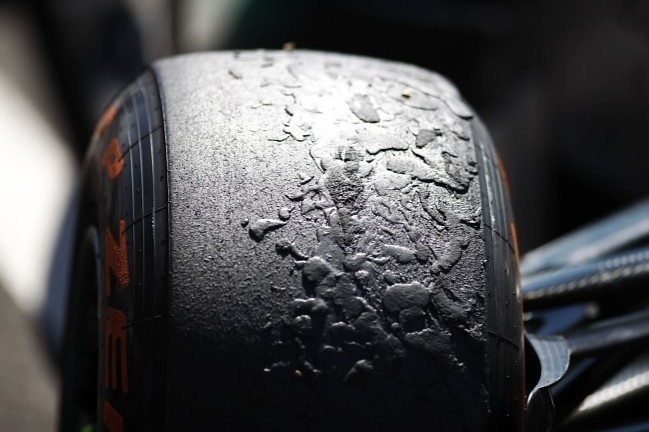
\includegraphics[width=\textwidth]{Figures/1_tyre_marbles.jpg}
    \caption{When a racer drivers over tyre marbles, the heat can cause them to attach to the tyre, causing it to be uneven and negatively impacting grip. Source: \cite{F1Technical2013TyreMarbles}. Reproduced for educational purposes only.}
    \label{image:tyre_marbles}
\end{figure}

\begin{figure}
    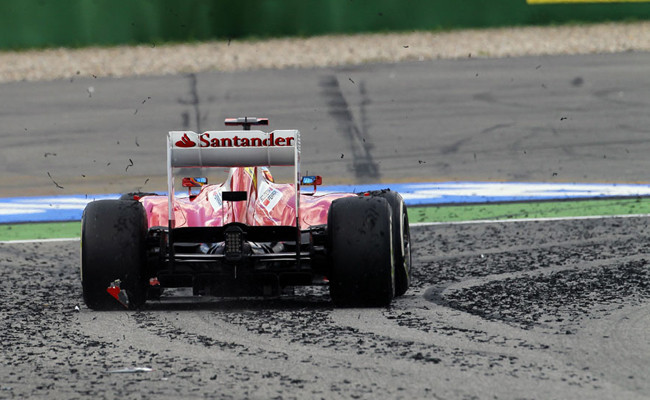
\includegraphics[width=\textwidth]{Figures/1_marbles_on_track.jpg}
    \caption{As the tyre degrades, chunks of rubber called marbles break off and start to collect off the racing line, typically on the outside of corners. Source: \cite{MotorPasion2014Marbles}. Reproduced for educational purposes only.}
    \label{image:track_marbles}
\end{figure}

The tyre is affected by mechanical and thermal degradation. Mechanical degradation refers to the physical characteristics of the tyre and how these wear due to repeated contact with the track. The tyre suffers significant shear forces (parallel to the surface) which cause parts of the material to slide against and alongside each other and remove rubber from the contact patch. This reduces the tyre's ability to conform the the microscopic grain of the racetrack surface and lowers the available grip \cite{Taylor2020FrictionRacingTyres}. The rate at which this occurs is influenced by several factors such as tyre compound, vehicle setup, driver inputs, track temperature, or circuit abrasiveness \cite{RacecarEngineering2020TyreGrip}. How each of these factors individually contributes is beyond the scope of this research, but the important consequence from a strategic perspective is that tyre grip degrades gradually throughout a race stint bringing a gradual reduction in lap time. Mechanical wear is generally progressive rather than instantaneous, meaning that over relatively short sections of a stint the associated loss of performance may be approximated using simplified degradation models. This assumption is explored further in Chapter 3 when selecting an appropriate representation for lap time prediction.

In parallel to this, thermal degradation describes the reduction in tyre performance caused by operating outside of its optimal operating window. The tyre builds temperature on the surface and inside the carcass as the tyre undergoes repeated cycles of braking, acceleration, and cornering. If the tyre exceeds its intended operational temperatures, the rubber compound in the tyre breaks down and loses its mechanical properties, causing reduced grip even if there is plenty of tyre rubber still available. Unlike purely mechanical wear, thermal degradation can therefore produce a noticeable reduction in performance without substantial physical loss of rubber.

In practice, tyre performance is rarely governed by a single degradation mechanism. Mechanical wear and thermal degradation occur simultaneously, with their relative importance varying according to the tyre compound, circuit characteristics, environmental conditions and driver behaviour. Rather than attempting to model these mechanisms independently, race strategy tools typically represent their combined effect through changes in lap time performance, as this is the quantity directly relevant to strategic decision making.

A racecar tyre typically shows four informally designated distinct phases of degradation over its lifetime \cite{Cappello2026TyreDegradation}, shown in \cref{fig:1_tyre_life} as a conceptual graph comparing age of the tyre in laps to a theoretical lap time in seconds. Each affects how the tyre behaves on the racetrack:
\begin{itemize}
    \item Ramping up: The tyre takes a small number of laps to reach its ideal operating temperature (lap 1-3). This process can be shortened by initially fitting the tyre at a higher temperature; F1 achieves this with tyre warming blanket which heat dry \& intermediate tyres to 70 degrees Celcius ({\degree}C) and wet tyres to 40 {\degree}C before being attached to the car.
    \item Peak Grip: The tyre is in its peak operating window (lap 3-15). Lap time degradation is slow and the tyre offers the best lap time. 
    \item Degradation: The tyre is no longer optimal, but is still providing competitive lap times (lap 15-45). The tyre will typically lose small amounts of lap time each lap, rather than hover around a consistent time. 
    \item The Cliff: The structural integrity of the tyre has failed and is essentially unusable for any competitive laps (lap 45 onwards). Lap times get much slower lap on lap and a puncture is not only risky but likely.
\end{itemize}

\begin{figure}[htbp]
\centering
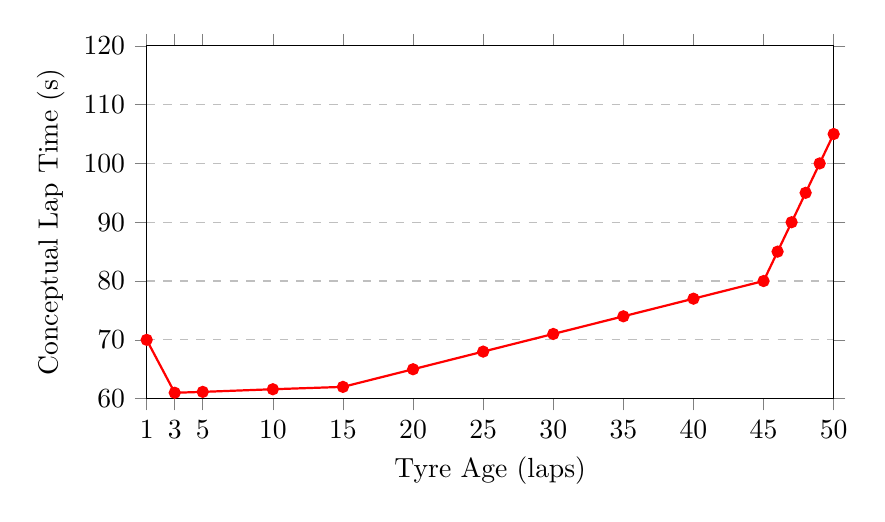
\begin{tikzpicture}
\begin{axis}[
    width=0.85\textwidth,
    height=0.5\textwidth,
    xlabel={Tyre Age (laps)},
    ylabel={Conceptual Lap Time (s)},
    xmin=1,
    xmax=50,
    ymin=60,
    ymax=120,
    ytick={60,70,80,90,100,110,120},
    xtick={1,3,5,10,15,20,25,30,35,40,45,50},
    ymajorgrids=true,
    grid style=dashed,
    legend style={
        at={(0.5,1.02)},
        anchor=south,
        legend columns=3,
        draw=none
    },
    tick align=outside
]

% Soft
\addplot[
    thick,
    red,
    mark=*,
    mark size=1.8pt
] coordinates {
(1,70)
(3,61)
(5,61.15)
(10,61.6)
(15,62)
(20,65)
(25,68)
(30,71)
(35,74)
(40,77)
(45,80)
(46,85)
(47,90)
(48,95)
(49,100)
(50,105)
};

\end{axis}
\end{tikzpicture}
\caption{Conceptual tyre degradation model of tyre lifecycle, demonstrating the four distinct phases of tyre behaviour - ramping up (laps 1-3), peak grip (laps 3-15), degradation (laps 15-45), and the cliff (laps 45-50).}
\label{fig:1_tyre_life}
\end{figure}

The impact of tyre degradation has a strong impact on choosing optimum pit stop times. A tyre that is rapidly degrading or approaching the final stage of its life significantly reduces the range of options for bringing the driver in for a tyre change. They need to be able to make the new tyre last until the end of the race or the intended stint. Pitting too many times will result in an unacceptable loss of race time even if the new tyres are theoretically much quicker. Strategists need to balance the physical tyre characteristics with the driver's abilities to control the behaviour of the tyre during its life to determine the ideal strategic option.

\subsection{Tyre Warm-Up and Out-Lap Performance}
\label{subsec:tyre-warmup-background}

% HIGH PRIORITY if warm-up is included in the model; MEDIUM otherwise.
% Explain why a newly fitted tyre may not deliver peak pace immediately.
% Relate this to undercut failure and overcut opportunity.
% Avoid implementation details and numerical assumptions here.

The out-lap is the first lap on a new tyre when leaving - or coming out of - the pit lane. This is one of the most critical periods of an undercut manoeuvre as the driver pitting driver needs to optimise their lap time so that, when the competitor does pit, they will come out behind. As discussed in \cref{subsec:tyre-degradation-background} the initial phase includes tyre warm-up to reach peak performance. This can result in failure to cut, resulting in an overcut for the defending driver where they manage to go longer with their stint and stay ahead.

In addition to the physical characteristics of the tyre, and how these change throughout a stint, the behaviour of the tyre can be controlled by the driver with their driving style or changes to the balance of the car. For example, a driver in a modern F1 car is able to adjust the balance of braking force longitudinally the car, meaning different amounts of braking forces are applied to front and rear tyres. The driver can also bring the tyre temperature to optimum faster with particular driving techniques, such as more pressure on the brakes to reduce the required braking distance. The sooner the tyre reaches peak performance, the best lap time the driver will have available for the crucial out-lap.

\section{Pit Stop Strategy Scenarios}
\label{sec:pit-stop-scenarios}

% PURPOSE: provide a common vocabulary for readers who may understand
% motorsport engineering but not race-strategy terminology.
% Keep each scenario concise and observational: what happens on track, what the
% team is trying to achieve, and which broad conditions favour it.

\subsection{Stay Out}
\label{subsec:stay-out}

% Explain:
% - the driver retains track position and continues on the current tyre;
% - potential reasons: clean air, avoiding traffic, extending to a preferred
%   compound/window, low degradation, or preserving strategic flexibility;
% - risks: worsening pace, exposure to an undercut, or reaching the tyre cliff.

\subsection{Undercut}
\label{subsec:undercut-background}

% Explain:
% - the attacking driver stops first;
% - the target remains on older tyres;
% - the attacker attempts to gain sufficient time before the target stops;
% - success is judged after the target's corresponding stop/rejoin.
% Mention broad favourable conditions: meaningful fresh-tyre delta, rapid
% warm-up, clear rejoin and sufficient offset time.
%
% SUGGESTED FIGURE 1.2 -- HIGH VALUE:
% A simple two-driver timeline showing pit order, offset laps and rejoin.

\subsection{Overcut}
\label{subsec:overcut-background}

% Explain:
% - the attacking/leading driver remains out after the rival stops;
% - it can work when old tyres remain competitive or the rival has a poor
%   out-lap, warm-up difficulty or traffic;
% - it is strategically relevant even if not a primary implemented output.
% Clarify later scope in Chapter \ref{chap:problem}.

\section{Existing Research and Modelling Approaches}
\label{sec:existing-research}

% VERY HIGH PRIORITY ACADEMIC SECTION.
% This is the integrated literature review thread. Direct papers specifically
% about F1 undercuts may be sparse; review the components instead:
% - race-strategy simulation and optimisation;
% - lap time and stint time modelling;
% - tyre degradation estimation from telemetry/timing data;
% - deterministic versus probabilistic strategy methods;
% - use of historical race data for validation.
%
% For each source, do more than summarise:
% - identify the method;
% - identify the useful contribution;
% - identify limitations for this project;
% - state how it informs the chosen approach.
%
% SUGGESTED TABLE 1.1:
% Source | Problem | Method | Relevant finding | Limitation / use here.
% This can efficiently demonstrate comparison rather than a source-by-source
% narrative.

[x - TODO - REVIEW AI WRITTEN TEXT]

Existing Formula One race strategy research has predominantly approached pit stop timing as a complete race optimisation problem. Proposed solutions range from discrete-event simulation and dynamic programming to
Monte Carlo planning, game theory and machine learning. Although these approaches differ in their treatment of uncertainty, competition and decision making, they share a common objective of determining an optimal
race strategy over an entire Grand Prix rather than evaluating an individual strategic opportunity.

Table \ref{tab:existing_research} summarises the principal approaches identified in the literature and their relevance to the present work.

\begin{table}[htbp]
\centering
\caption{Comparison of Formula One race strategy modelling approaches.}
\label{tab:existing_research}

\small
\renewcommand{\arraystretch}{1.25}

\begin{tabularx}{\textwidth}{|
>{\raggedright\arraybackslash}p{0.21\textwidth}|
>{\raggedright\arraybackslash}p{0.18\textwidth}|
>{\raggedright\arraybackslash}p{0.16\textwidth}|
X|
}
\hline
\textbf{Source}
&
\textbf{Method}
&
\textbf{Scope}
&
\textbf{Relevance to this project}
\\
\hline

Bekker \& Lotz
\cite{BekkerLotz2009}
&
Discrete-event simulation
&
Whole-race strategy
&
Demonstrates historical race simulation and validation against real race outcomes, supporting the use of simulation as a decision-support tool.
\\
\hline

Carrasco Heine \& Thraves
\cite{CarrascoHeineThraves2023}
&
Dynamic programming
&
Whole-race optimisation
&
Models tyre wear and cumulative race time. Supports lap time based optimisation but not isolated undercut analysis.
\\
\hline

Piccinotti
\cite{Piccinotti2021}
&
Monte Carlo planning
&
Whole-race planning
&
Uses historical race data and probabilistic simulation to evaluate strategic options under uncertainty.
\\
\hline

Aguad \& Thraves
\cite{AguadThraves2024}
&
Dynamic programming and game theory
&
Two-driver interaction
&
Introduces direct interaction between competing drivers, conceptually similar to the two-driver comparison considered in this work.
\\
\hline

Thomas et al.
\cite{ThomasEtAl2025}
&
Explainable reinforcement learning
&
Whole-race optimisation
&
Demonstrates modern AI-based strategy optimisation while maintaining model interpretability.
\\
\hline

Hettmann
\cite{Hettmann2024}
&
Machine learning
&
Pit stop prediction
&
Predicts pit stop timing from historical races rather than evaluating the engineering causes of successful undercuts.
\\
\hline

Fatima \& Johrendt
\cite{FatimaJohrendt2023}
&
Deep neural networks
&
Race outcome prediction
&
Illustrates the increasing application of deep learning to Formula One strategy, although with limited transparency.
\\
\hline

\end{tabularx}

\end{table}

The earliest work identified is that of Bekker and Lotz \cite{BekkerLotz2009}, who demonstrated that Formula One race strategy could be represented using discrete-event simulation. Their model incorporated pit stops, overtaking and race interruptions before validating the resulting simulator against three historic Grands Prix. Although based on regulations that pre-date the modern tyre-focused era, the work established simulation as a viable methodology for evaluating race strategy using historical data.

Subsequent research has generally shifted towards optimisation rather than simulation alone. Carrasco Heine and Thraves \cite{CarrascoHeineThraves2023} formulate race strategy as a dynamic programming problem, minimising cumulative race time while accounting for tyre degradation, compound selection and stochastic events such as yellow flags. Aguad and Thraves \cite{AguadThraves2024} extend this concept by modelling strategic interaction between competing drivers using a Stackelberg feedback game. These approaches demonstrate that race strategy can be formulated as a mathematical optimisation problem but are primarily concerned with determining globally optimal race strategies rather than evaluating an individual undercut opportunity.

More recent work has increasingly adopted machine learning techniques. Hettmann \cite{Hettmann2024} predicts pit stop timing using supervised learning and driver clustering, while Fatima and Johrendt \cite{FatimaJohrendt2023} employ deep neural networks to predict race outcomes and strategic decisions. Thomas et al. \cite{ThomasEtAl2025} further demonstrate that reinforcement learning can produce competitive race strategies while retaining a degree of interpretability through explainable artificial intelligence techniques. These approaches illustrate the predictive capability of data-driven models but generally sacrifice the transparency offered by deterministic engineering models.

A complementary direction is represented by Piccinotti \cite{Piccinotti2021}, who combines historical Formula One data with Monte Carlo simulation to explore race strategies under uncertainty. By sampling many possible race evolutions, the model accounts for uncertainty in competitor behaviour and race events. This probabilistic approach contrasts with the present work, which deliberately considers a deterministic retrospective scenario in which the observed race provides the complete set of external conditions.

Collectively, these studies demonstrate that Formula One race strategy has been successfully modelled using a wide range of optimisation, simulation and machine learning techniques. However, the overwhelming majority seek to optimise or predict complete race strategies. Relatively little attention has been given to the isolated engineering problem of evaluating whether a specific undercut opportunity existed at a particular point during a race.

Consequently, this dissertation adopts a deliberately narrower scope. It does not attempt to determine the globally optimal race strategy or predict competitor behaviour. Instead, it develops a transparent, deterministic model that compares two observed drivers over a local decision window, allowing the contribution of tyre degradation, compound performance, warm-up effects and traffic to be examined individually. This positions the work between descriptive historical analysis and complete race-strategy optimisation while maintaining direct interpretability of every modelling assumption.

[x - TODO - REVIEW AI WRITTEN TEXT]

\section{Research Gap and Project Motivation}
\label{sec:research-gap}

% VERY HIGH PRIORITY -- final section of Chapter 1.
% Synthesise the literature and context into a clear gap. Avoid claiming that
% no undercut tools exist unless this can be evidenced.
%
% A defensible framing might be:
% - professional teams use sophisticated proprietary strategy systems;
% - public research often treats whole-race optimisation or individual tyre
%   effects rather than an explainable undercut-focused comparison;
% - there is value in a transparent, configurable and historically validated
%   model showing how individual assumptions affect predicted undercut gain.
%
% End with a transition to Chapter \ref{chap:problem}, which formalises the aim,
% objectives, scope and success criteria.

The preceding sections demonstrate that Formula One race strategy has received considerable academic attention. Existing work has successfully applied discrete-event simulation, dynamic programming, game theory, Monte Carlo methods and machine learning to optimise race strategy, predict pit stop timing and improve race outcomes. These studies demonstrate that race strategy is a suitable domain for mathematical modelling and provide a strong methodological foundation for future research.

Despite this breadth of research, the majority of published work treats pit stop timing as part of a complete race optimisation problem. Simulation models generally seek to determine an optimal race strategy, while machine learning approaches attempt to predict competitor actions or race outcomes. Consequently, comparatively little attention has been given to analysing individual strategic opportunities within an observed race using a transparent and explainable engineering model.

The undercut represents one of the most influential tactical decisions available during a Formula One race. While its effectiveness is widely recognised within professional motorsport, evaluating whether an undercut opportunity genuinely existed requires consideration of tyre degradation, compound performance, warm-up behaviour, traffic and other interacting factors. Existing optimisation frameworks naturally include many of these effects, but they do not typically isolate the undercut as an engineering problem in its own right or provide clear visibility of how individual assumptions influence the predicted outcome.

This dissertation therefore adopts a deliberately narrower scope than much of the existing literature. Rather than predicting complete race strategies or replacing the judgement of race engineers, it develops a deterministic model that evaluates historical undercut opportunities between two observed drivers. By exposing the principal modelling parameters and validating the resulting predictions against historical race data, the model provides a transparent framework through which the effect of individual engineering  assumptions can be examined and understood.

The remainder of this dissertation formalises this objective. Chapter \ref{chap:problem} defines the research aims, objectives, project scope and success criteria before introducing the assumptions that underpin the proposed modelling approach.